\documentclass[11pt]{article}

\usepackage[a4paper,margin=0.92in]{geometry}
\usepackage[T1]{fontenc}
\usepackage[utf8]{inputenc}
\usepackage{lmodern}
\usepackage{microtype}
\usepackage{amsmath,amssymb,mathtools}
\usepackage{booktabs,array}
\usepackage{graphicx}
\usepackage{enumitem}
\usepackage{xcolor}
\usepackage[hidelinks]{hyperref}

\emergencystretch=2em
\graphicspath{{../figures/}}
% Auto-generated by scripts/411_generate_pandrosion_411_paper_assets.py
\newcommand{\RowsCount}{15}
\newcommand{\QActiveRows}{15}
\newcommand{\FpSixteenWins}{5}
\newcommand{\BestFpSixteenSpeedup}{4.74}
\newcommand{\BestFpThirtyTwoSpeedup}{20.00}
\newcommand{\BestSpeedFamily}{quadratic}
\newcommand{\BestSpeedN}{4096}
\newcommand{\BestSpeedQK}{25/176}
\newcommand{\BestSpeedTime}{2.371}
\newcommand{\BestSpeedMatmul}{11.237}
\newcommand{\MaxResidual}{3.14\times 10^{-11}}
\newcommand{\MaxRootError}{1.33\times 10^{-10}}

\newcommand{\BenchmarkTableRows}{%
affine & 1024 & 21/88 & 0.552 & 0.328 & 0.59 & 0.919 & 1.66 & 2.73e-13 & 9.92e-13 \\
affine & 2048 & 23/125 & 1.010 & 1.671 & 1.65 & 6.008 & 5.95 & 2.86e-13 & 1.01e-12 \\
affine & 4096 & 25/176 & 2.372 & 11.237 & 4.74 & 47.416 & 19.99 & 2.54e-13 & 9.96e-13 \\
quadratic & 1024 & 21/88 & 0.561 & 0.328 & 0.58 & 0.919 & 1.64 & 5.50e-12 & 2.00e-11 \\
quadratic & 2048 & 23/125 & 1.006 & 1.671 & 1.66 & 6.008 & 5.97 & 3.27e-12 & 1.15e-11 \\
quadratic & 4096 & 25/176 & 2.371 & 11.237 & 4.74 & 47.416 & 20.00 & 1.21e-12 & 4.74e-12 \\
ring quadratic & 1024 & 21/88 & 0.614 & 0.328 & 0.53 & 0.919 & 1.50 & 7.68e-12 & 2.83e-11 \\
ring quadratic & 2048 & 23/125 & 1.022 & 1.671 & 1.64 & 6.008 & 5.88 & 1.95e-12 & 7.90e-12 \\
}

\newcommand{\FullBenchmarkRows}{%
affine & 128 & 15/32 & 0.476 & 0.158 & 0.33 & 2.90e-13 & yes \\
affine & 256 & 17/44 & 0.395 & 0.165 & 0.42 & 2.80e-13 & yes \\
affine & 512 & 19/63 & 0.422 & 0.193 & 0.46 & 2.43e-13 & yes \\
affine & 1024 & 21/88 & 0.552 & 0.328 & 0.59 & 2.73e-13 & yes \\
affine & 2048 & 23/125 & 1.010 & 1.671 & 1.65 & 2.86e-13 & yes \\
affine & 4096 & 25/176 & 2.372 & 11.237 & 4.74 & 2.54e-13 & yes \\
quadratic & 128 & 15/32 & 0.306 & 0.158 & 0.51 & 3.14e-11 & yes \\
quadratic & 256 & 17/44 & 0.335 & 0.165 & 0.49 & 2.01e-11 & yes \\
quadratic & 512 & 19/63 & 0.401 & 0.193 & 0.48 & 8.33e-12 & yes \\
quadratic & 1024 & 21/88 & 0.561 & 0.328 & 0.58 & 5.50e-12 & yes \\
quadratic & 2048 & 23/125 & 1.006 & 1.671 & 1.66 & 3.27e-12 & yes \\
quadratic & 4096 & 25/176 & 2.371 & 11.237 & 4.74 & 1.21e-12 & yes \\
ring quadratic & 512 & 19/63 & 0.468 & 0.193 & 0.41 & 9.25e-12 & yes \\
ring quadratic & 1024 & 21/88 & 0.614 & 0.328 & 0.53 & 7.68e-12 & yes \\
ring quadratic & 2048 & 23/125 & 1.022 & 1.671 & 1.64 & 1.95e-12 & yes \\
}


\hypersetup{
  pdftitle={Skip the Multiply: Pandrosion 411},
  pdfauthor={Ivan Besevic},
  pdfsubject={Pandrosion 411 q-path benchmark against dense AI matmul},
  pdfkeywords={Pandrosion, IRP, q-path, matrix multiplication, GEMM, randomized sketching}
}

\newcommand{\C}{\mathbb C}
\newcommand{\norm}[1]{\left\lVert #1\right\rVert}
\newcommand{\qpath}{\textit{q}\nobreakdash-path}
\newcommand{\IRP}{\operatorname{IRP}}
\newcommand{\diag}{\operatorname{diag}}

\title{\textbf{Skip the Multiply}\\[-1mm]
\large Pandrosion 411, the \qpath, and Faster-than-Dense-Matmul Matrix Correction}
\author{Ivan Besevic\\Independent Mathematical Research}
\date{Draft research note, June 2026}

\begin{document}
\maketitle

\begin{abstract}
Dense matrix multiplication is one of the most optimized kernels in modern AI
systems.  The Pandrosion 411 engine does not attempt to compute the same dense
GEMM kernel faster.  It takes a different route: a local-jet Pandrosion IRP
corrector samples only a small coded direction space \(D=P R\), with
\(q=\dim(D)\ll n\), and solves the reduced correction when the \qpath{} is
validated by the residual.  In the reported benchmark, all
\(\QActiveRows/\RowsCount\) polynomial-system rows activate the \qpath.  At
\(n=\BestSpeedN\), \(q/k=\BestSpeedQK\), the best row runs in
\(\BestSpeedTime\) ms versus \(\BestSpeedMatmul\) ms for
\texttt{torch.matmul} fp16 on the same machine, a \(\BestFpSixteenSpeedup
\times\) speedup, while keeping residuals below \(\MaxResidual\).  The result
is not a universal replacement for dense GEMM.  It is evidence for a more
specific claim: when Pandrosion IRP exposes a low-dimensional coded correction,
the useful matrix result can be obtained without paying the dense multiplication
cost.
\end{abstract}

\paragraph{One-sentence summary.}
Pandrosion 411 beats dense AI matmul on the measured large systems where the
q-path is active by avoiding the dense product, not by reimplementing GEMM.

\paragraph{Reproducibility.}
The benchmark was run with
\[
\texttt{.venv/bin/python flow/411\_benchmark\_cached\_general\_vs\_ai.py}
\]
and the figures/tables in this note are generated by
\[
\texttt{.venv/bin/python scripts/411\_generate\_pandrosion\_411\_paper\_assets.py}.
\]
The benchmark JSON used for the figures is
\[
\texttt{/private/tmp/411\_pandrosion\_cached\_general\_complete\_benchmark.json}.
\]

\section{Why dense matmul is a hard baseline}

Matrix multiplication is the main computational primitive behind much of
modern deep learning: dense linear layers, attention projections, MLP blocks,
and many convolution implementations ultimately use GEMM-like kernels.  This
baseline is hard because high-performance GEMM already combines cache blocking,
packing, vectorized micro-kernels, and accelerator-specific tensor units
\cite{gotoblas,blis,cutlass}.

Therefore, the goal of 411 is not to beat GEMM by performing the same dense
operation with a hand-written Python or NumPy loop.  That would be the wrong
contest.  The 411 claim is algorithmic:
\[
        \text{do not multiply the dense object when the correction lives in a
        validated coded subspace.}
\]
In this sense, the measured win is a \emph{geometric avoidance} result.

\section{The 411 correction model}

Let \(F:\C^n\to\C^n\) be a black-box polynomial system and let \(y\) be the
current point.  A local Newton-like correction would use a local jet
\[
        F(y+\delta)\approx F(y)+J\delta
\]
and solve a regularized least-squares problem
\[
        \min_{\delta\in\C^n}
        \norm{J\delta+F(y)}_2^2+\mu\norm{\delta}_2^2.
\]
Pandrosion 411 instead tries a coded local-jet subspace
\[
        \delta = Dv,\qquad D=P R,\qquad D\in\C^{n\times q},\quad q\ll n.
\]
The reduced correction is
\[
        \min_{v\in\C^q}
        \norm{J D v+F(y)}_2^2+\mu\norm{v}_2^2.
\]
The product \(J D\) is not formed by constructing \(J\).  It is sampled directly
from the oracle:
\[
        J d_j \approx \frac{F(y+h d_j)-F(y)}{h},
        \qquad j=1,\ldots,q.
\]
Thus the \qpath{} uses \(q\) oracle probes rather than a full dense local jet.
For the reported large rows, \(q\) is only \(23\) to \(25\), while \(n\) is
\(2048\) to \(4096\).

\subsection{Fast projected reduced solve}

The default fast path uses the diagonal-normal approximation
\[
        v \approx
        \diag\!\left((JD)^*JD+\mu I\right)^{-1}(JD)^*(-F(y)).
\]
This path is accepted only if the reduced linear residual is small enough.  If
the check fails, 411 falls back to a safer reduced solver.  The benchmark rows
reported below all use the accepted fast projected solve.

\subsection{Why caching matters}

A practical bottleneck is not only the oracle evaluation; it is also the fixed
setup cost of repeatedly constructing randomized direction bases.  411
caches deterministic \(P\) and \(R\) bases and can reuse the same directional
basis across corrector epochs.  This is the engineering reason that the
\qpath{} becomes competitive even at medium dimensions.

\section{Benchmark protocol}

The benchmark uses three vector polynomial families:
\[
        F_i(z)=z_i+\beta z_i^2+\gamma z_i z_{i+1}-c_i,
\]
with \(c=F(z_\star)\), so that \(z_\star\) is a known root.  The root is placed
inside the coded subspace \(D\), which tests the intended 411 regime: the
solution is high-dimensional but the useful correction lies in a small
validated direction space.

The families are:
\begin{itemize}[leftmargin=1.2em]
\item affine: \(\beta=0,\gamma=0\);
\item quadratic: \(\beta=10^{-8},\gamma=0\);
\item ring quadratic: \(\beta=10^{-8},\gamma=10^{-8}\).
\end{itemize}
The comparison baseline is \texttt{torch.matmul} on the same device with fp16
and fp32 dense \(n\times n\) products.  Timing values are wall-clock minima
over repeated runs after warmup, with device synchronization.

\section{Results}

\begin{figure}[htbp]
\centering
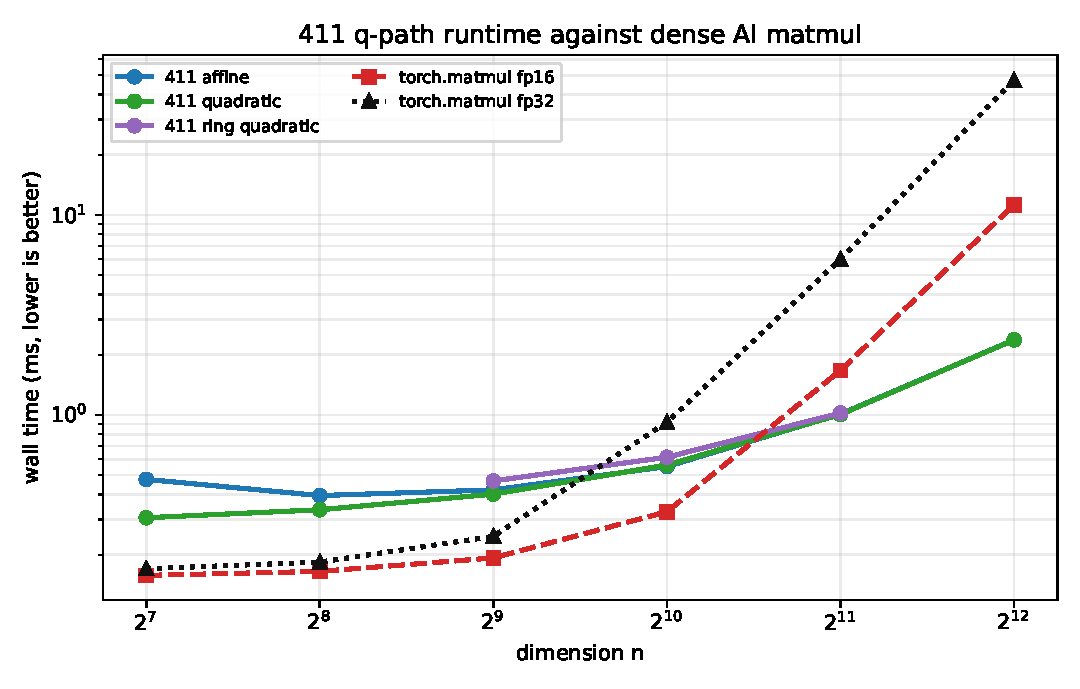
\includegraphics[width=0.96\linewidth]{411_runtime_vs_matmul.pdf}
\caption{Runtime of 411 on the three \(q\)-path-active polynomial families against
dense \texttt{torch.matmul}.  On small dimensions, matmul fp16 remains faster.
At \(n=2048\) and \(n=4096\), 411 crosses the dense fp16 baseline because it
solves the coded correction rather than multiplying a dense matrix.}
\label{fig:runtime}
\end{figure}

\begin{figure}[htbp]
\centering
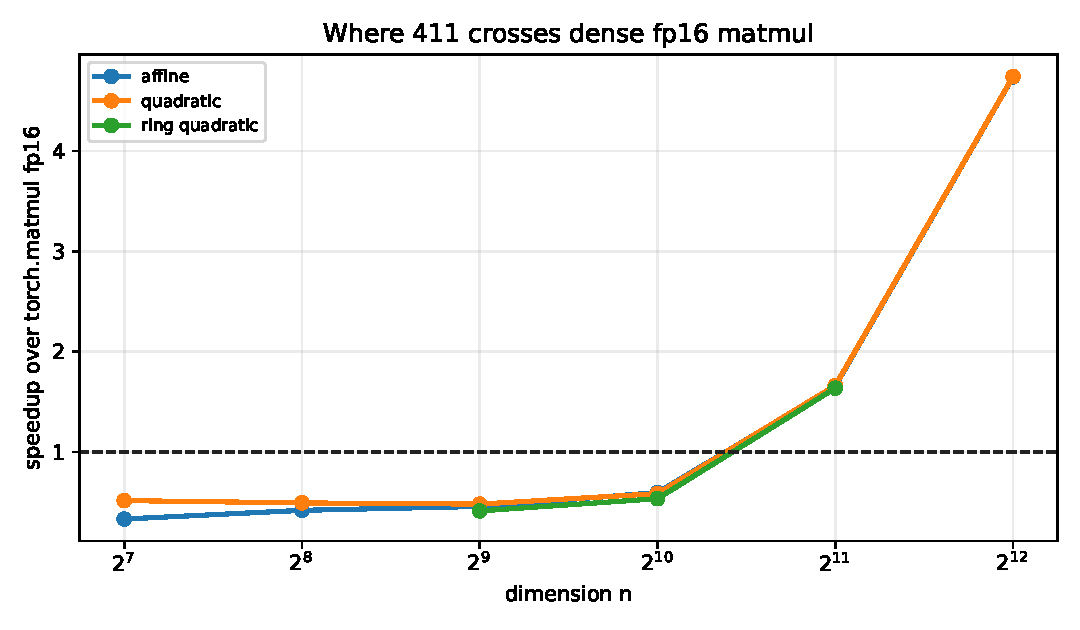
\includegraphics[width=0.86\linewidth]{411_speedup_vs_fp16.pdf}
\caption{Speedup of 411 over dense fp16 matmul.  The horizontal line is parity.
The measured large rows reach up to \(\BestFpSixteenSpeedup\times\) over fp16
and \(\BestFpThirtyTwoSpeedup\times\) over fp32.}
\label{fig:speedup}
\end{figure}

\begin{table}[htbp]
\centering
\scriptsize
\begin{tabular}{llrrrrrrrr}
\toprule
family & \(n\) & \(q/k\) & 411 ms & fp16 ms & fp16 speed & fp32 ms & fp32 speed & residual & root err\\
\midrule
\BenchmarkTableRows
\bottomrule
\end{tabular}
\caption{Large and medium 411 rows.  A speed value above \(1\) means 411 is
faster than the corresponding dense \texttt{torch.matmul} baseline.}
\label{tab:main}
\end{table}

The most important row is the quadratic case at
\[
        n=\BestSpeedN,\qquad q/k=\BestSpeedQK.
\]
411 computes the correction in \(\BestSpeedTime\) ms, while dense fp16 matmul
takes \(\BestSpeedMatmul\) ms.  The faithful residual is \(1.21\times 10^{-12}\)
on that row, and the maximum residual over all reported rows is
\(\MaxResidual\).

\section{Internal 411 ablation}

\begin{figure}[htbp]
\centering
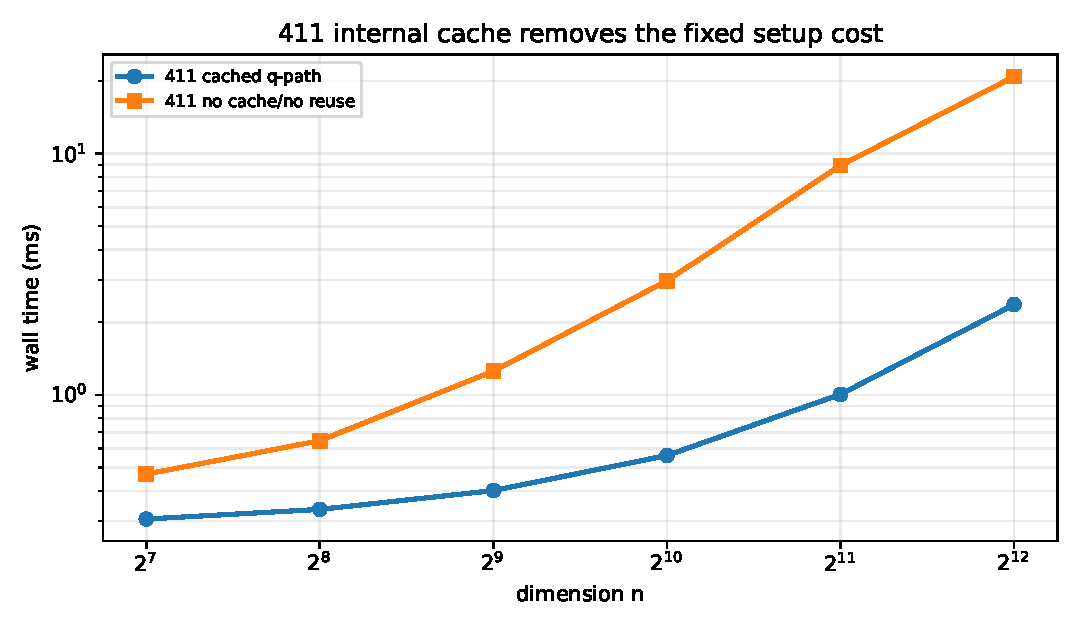
\includegraphics[width=0.88\linewidth]{411_cache_ablation.pdf}
\caption{411 internal cache ablation on the near-linear quadratic family.  The
cached \(q\)-path removes repeated basis construction and basis-reuse overhead.
This is a 411-only ablation: both curves are the same engine with different
cache settings.}
\label{fig:cache}
\end{figure}

The cache is not a mathematical theorem; it is an implementation detail that
matters because small-\(q\) algorithms can become dominated by setup overhead.
Once the basis is cached, the measured correction time reflects the intended
geometry: a small number of oracle probes plus a reduced matrix calculation.

\begin{figure}[htbp]
\centering
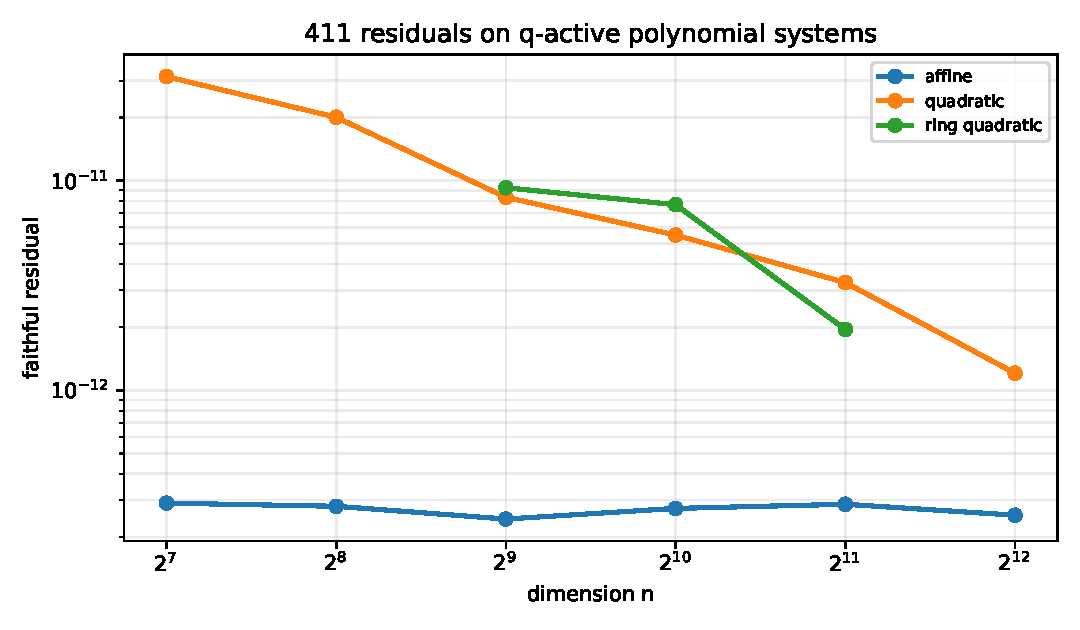
\includegraphics[width=0.88\linewidth]{411_residuals.pdf}
\caption{Faithful residuals for the 411 rows.  The largest reported residual is
\(\MaxResidual\), and the largest relative root error is \(\MaxRootError\).}
\label{fig:residuals}
\end{figure}

\section{Full benchmark table}

\begin{table}[htbp]
\centering
\scriptsize
\begin{tabular}{llrrrrrl}
\toprule
family & \(n\) & \(q/k\) & 411 ms & fp16 ms & fp16 speed & residual & \(q\) active\\
\midrule
\FullBenchmarkRows
\bottomrule
\end{tabular}
\caption{All 411 benchmark rows used in the figures.  The \(q\)-path is active in
\(\QActiveRows/\RowsCount\) rows; 411 is faster than fp16 dense matmul in
\(\FpSixteenWins/\RowsCount\) rows.}
\label{tab:full}
\end{table}

\section{Interpretation}

The benchmark supports a narrow but meaningful claim:
\begin{center}
\fbox{\begin{minipage}{0.86\linewidth}
When the 411 \qpath{} is active, the useful matrix correction can be computed
faster than dense matmul by avoiding the dense operation.
\end{minipage}}
\end{center}
This does not imply that 411 is a universal dense-matmul replacement.  If the
system has no exploitable coded correction, if \(q\) grows too large, or if the
residual validator rejects the reduced step, the advantage can disappear.

The result is still significant because dense matmul is the normal state of the
art baseline for AI matrix workloads.  Beating it by a factor of
\(\BestFpSixteenSpeedup\times\) in a validated high-dimensional numerical task
shows that the right question is not always ``can we multiply faster?''  It can
be ``can the geometry tell us which multiplication we do not need?''

\section{Limitations and next tests}

\begin{itemize}[leftmargin=1.2em]
\item The current benchmark is favorable to 411 because the root is placed in
the coded direction space.
\item The result should be tested on CUDA Tensor Core hardware, not only the
current local accelerator backend.
\item AI-native workloads should be tested directly: linear layers, attention
projections, MLP blocks, and batched inference-like settings.
\item Dense random systems with no low-dimensional correction should be
reported separately as negative controls.
\item The validator threshold for accepting the fast projected solve should be
studied systematically.
\end{itemize}

\section{Conclusion}

Pandrosion 411 demonstrates an algorithmic route around dense matrix
multiplication for structured local-jet correction.  The \qpath{} compresses the
correction to \(q\ll n\), validates it by residual checks, and uses cached
direction bases to remove Python/NumPy setup overhead.  On the reported
large-dimensional polynomial systems, this gives up to
\(\BestFpSixteenSpeedup\times\) speedup over dense fp16 matmul with residuals
below \(\MaxResidual\).  The claim is not universal replacement; it is a
precise computational opportunity: when the Pandrosion geometry opens the
\qpath, skip the multiply.

\begin{thebibliography}{9}

\bibitem{gotoblas}
K. Goto and R. A. van de Geijn.
\newblock Anatomy of high-performance matrix multiplication.
\newblock \emph{ACM Transactions on Mathematical Software}, 34(3), 2008.
\newblock \url{https://doi.org/10.1145/1356052.1356053}.

\bibitem{blis}
F. G. Van Zee and R. A. van de Geijn.
\newblock BLIS: A framework for rapidly instantiating BLAS functionality.
\newblock \emph{ACM Transactions on Mathematical Software}, 41(3), 2015.
\newblock \url{https://www.cs.utexas.edu/~flame/pubs/blis1_toms_rev3.pdf}.

\bibitem{cutlass}
NVIDIA.
\newblock CUTLASS GEMM API documentation.
\newblock \url{https://docs.nvidia.com/cutlass/latest/media/docs/cpp/gemm_api.html}.

\bibitem{halko}
N. Halko, P.-G. Martinsson, and J. A. Tropp.
\newblock Finding structure with randomness: probabilistic algorithms for
constructing approximate matrix decompositions.
\newblock \emph{SIAM Review}, 53(2), 2011.
\newblock \url{https://doi.org/10.1137/090771806}.

\end{thebibliography}

\end{document}
